\chapter{Evaluation of the stable Autoencoder}



\section{DRAFT}
% ── Q2b stable ───────────────────────────────────────────────
\begin{figure}[H]
    \centering
    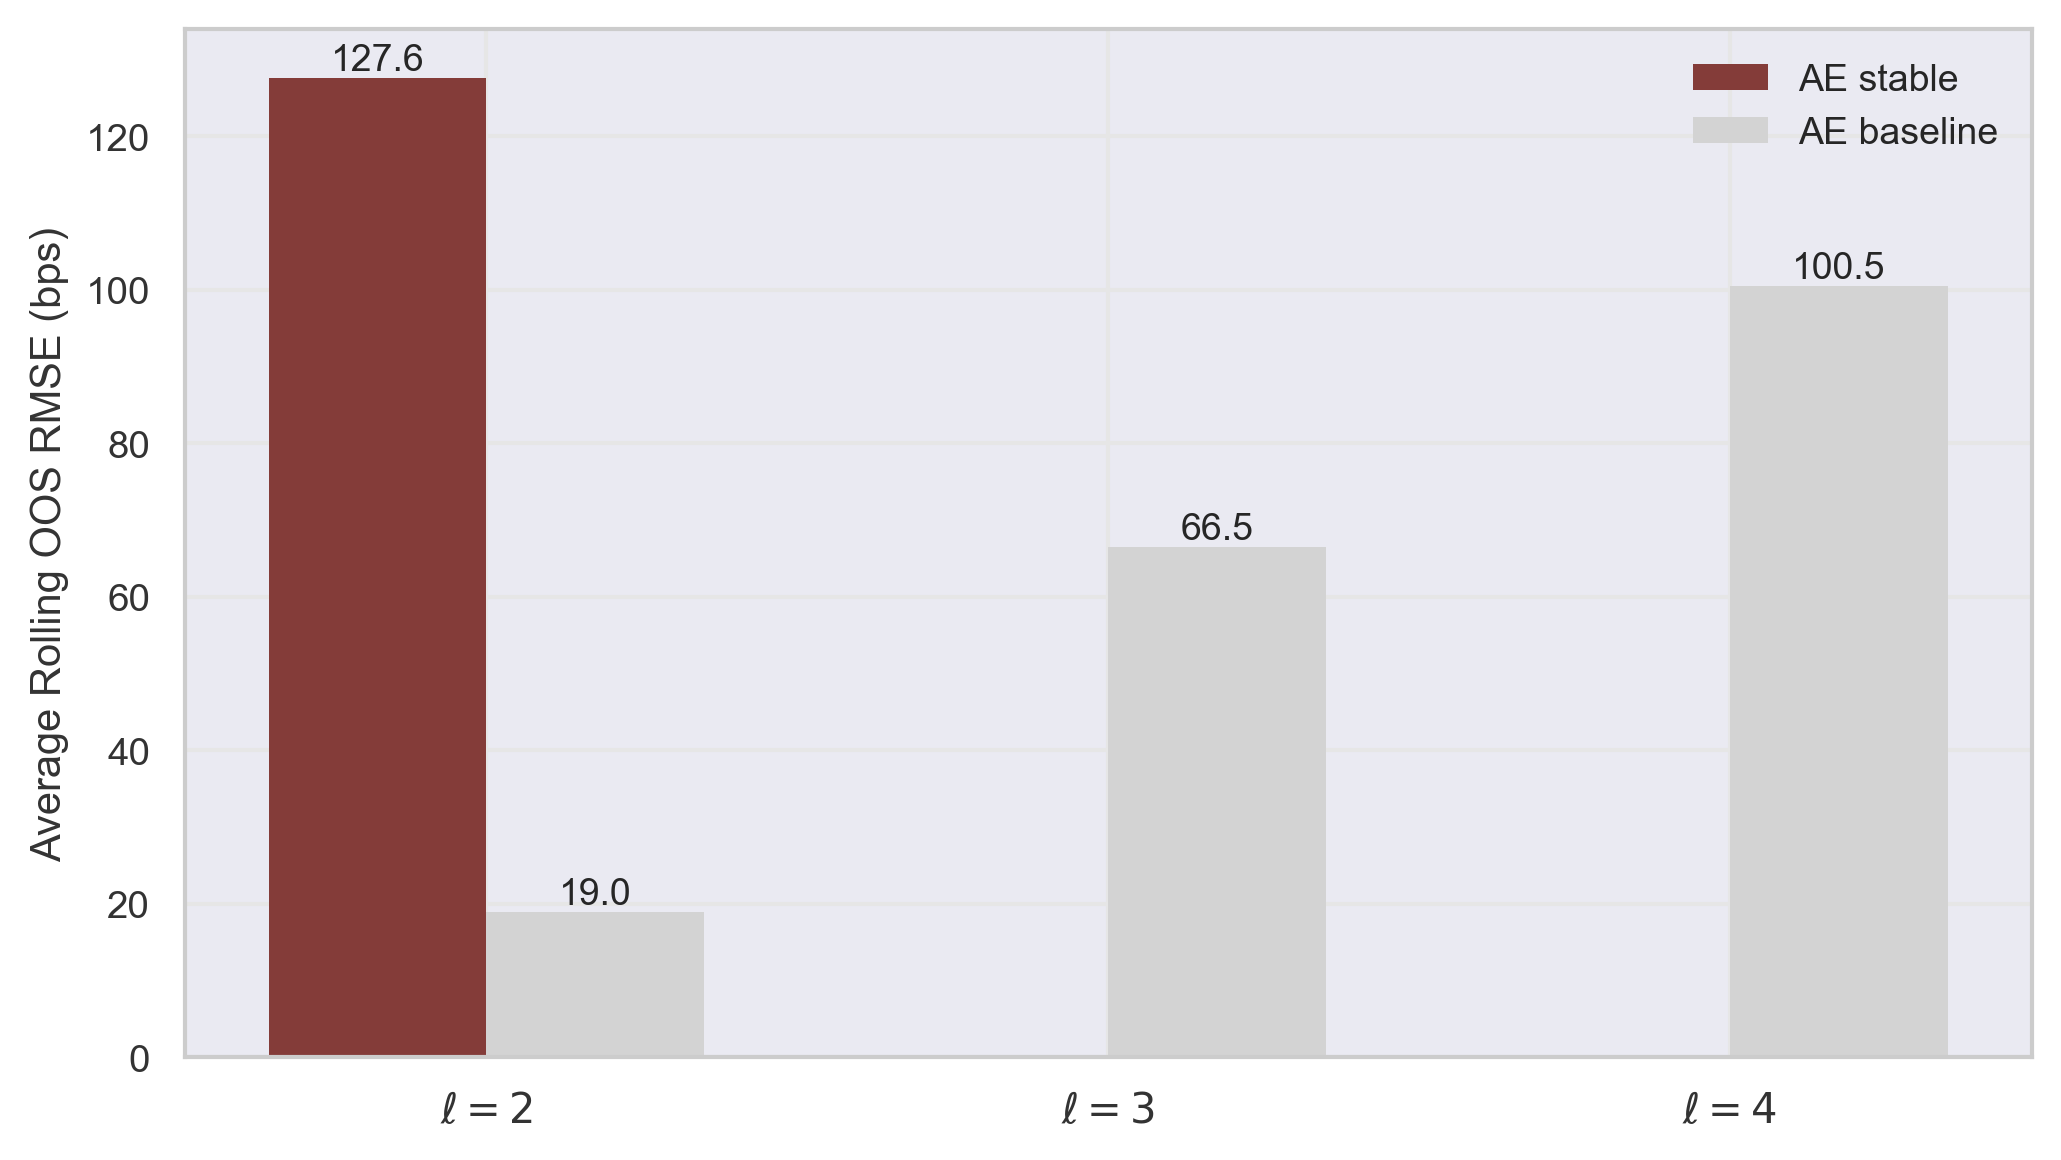
\includegraphics[width=0.75\textwidth]{Figures/thesis_results/AutoencoderPerformanceStable/Q2b_rolling_oos_vs_dim_stable.png}
    \caption{Average rolling out-of-sample RMSE (bps) for the stable autoencoder and the
    EKF DNS benchmark across latent dimensions $\ell \in \{2, 3, 4\}$.
    Autoencoder bars are coloured by model:
    $\ell=2$ ({\color[HTML]{843C39}\rule[0.5ex]{1em}{1.5pt}}),
    $\ell=3$ ({\color[HTML]{393B79}\rule[0.5ex]{1em}{1.5pt}}),
    $\ell=4$ ({\color[HTML]{D6616B}\rule[0.5ex]{1em}{1.5pt}}).
    EKF DNS bars are shown in grey.
    Values are averaged across all valid rolling windows.}
    \label{fig:Q2b_stable}
\end{figure}

% ── Q3b stable ───────────────────────────────────────────────
\begin{figure}[H]
    \centering
    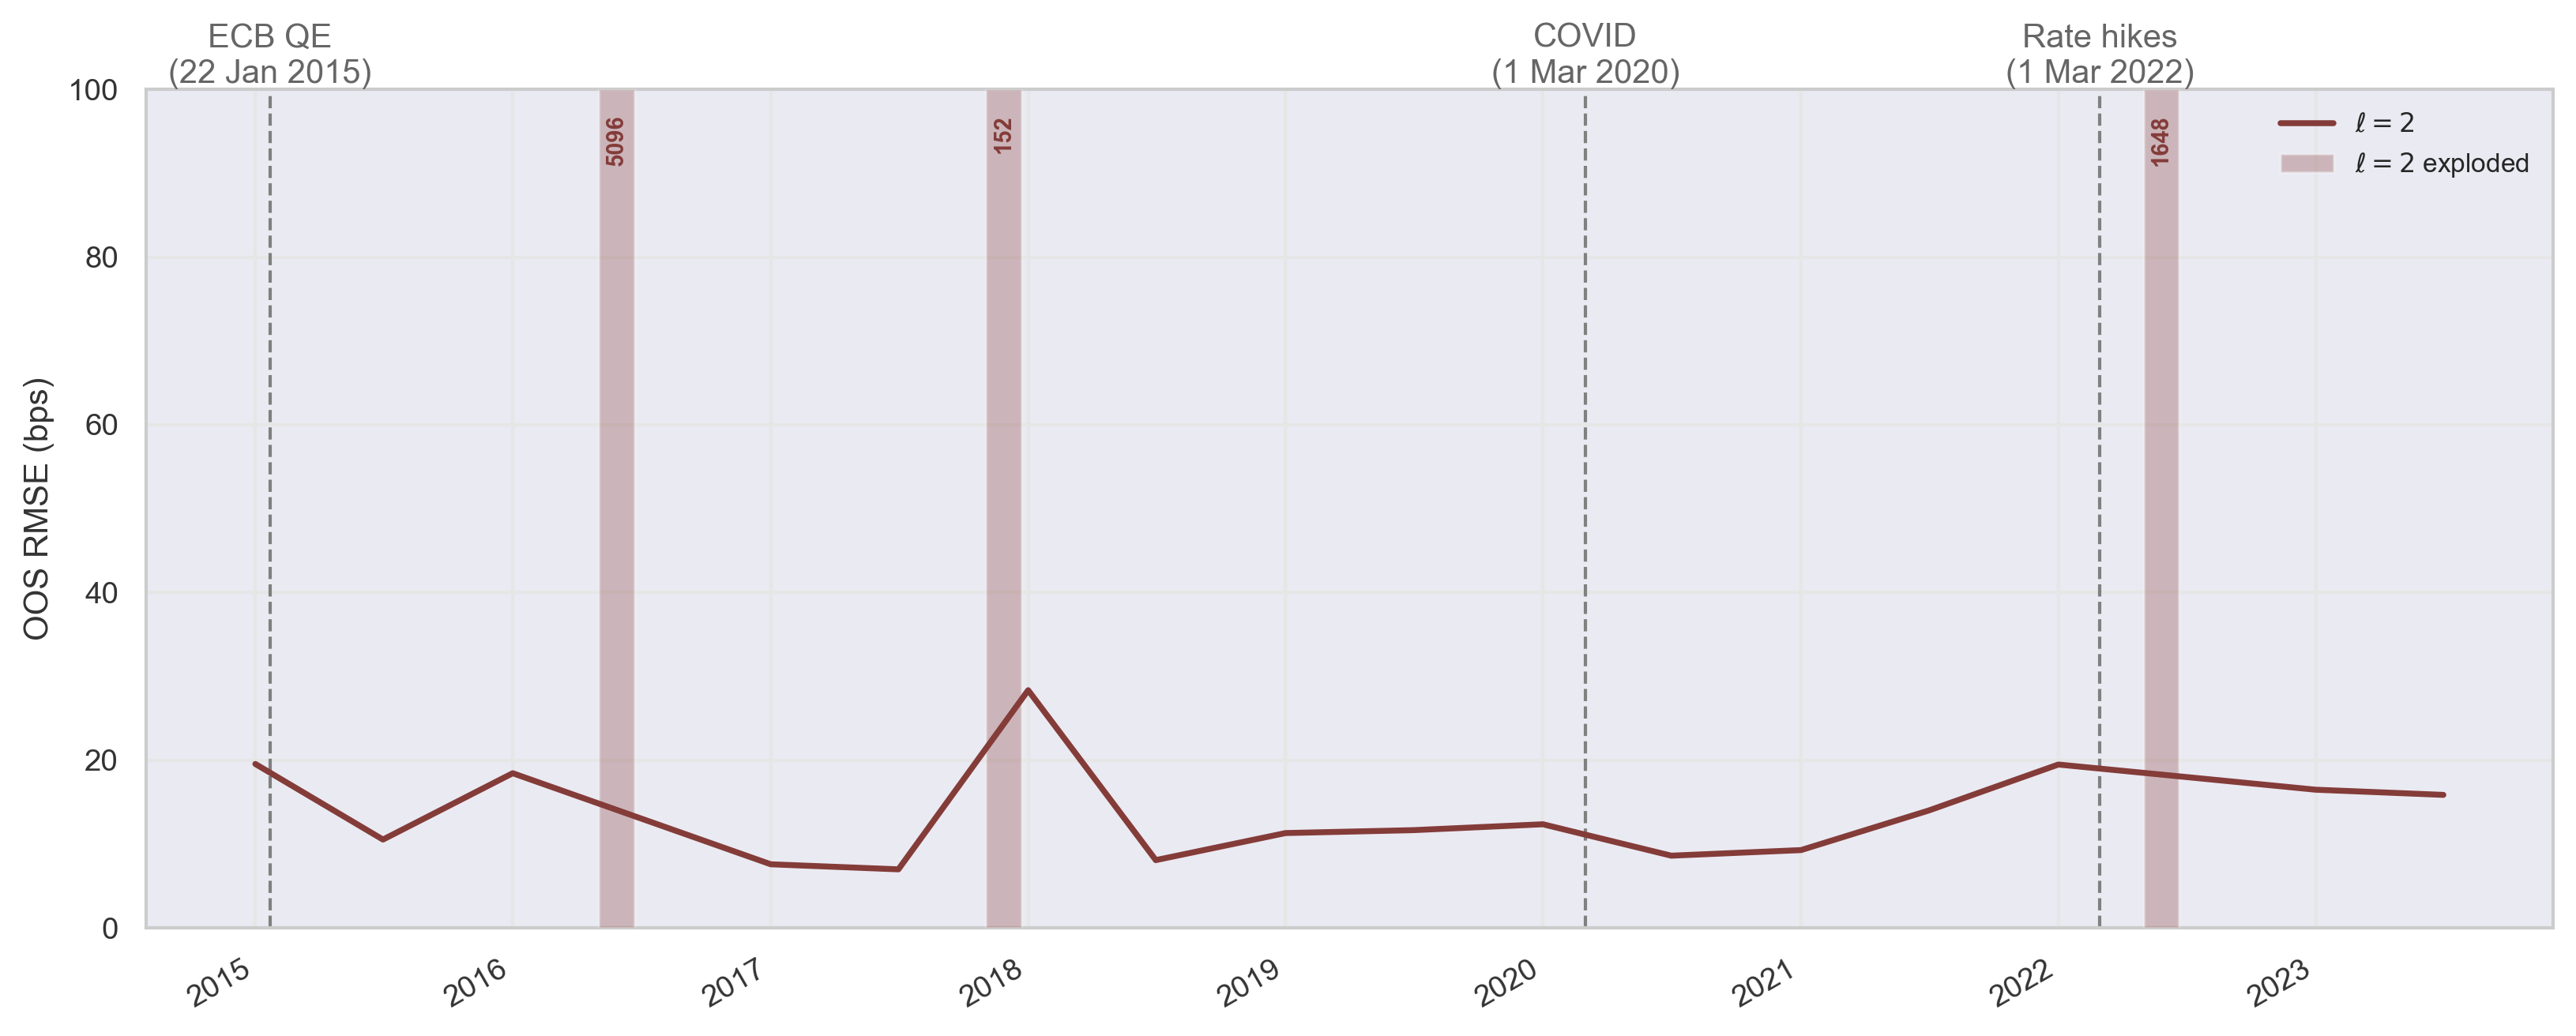
\includegraphics[width=1.0\textwidth]{Figures/thesis_results/AutoencoderPerformanceStable/Q3b_rolling_rmse_over_time_stable.png}
    \caption{Rolling out-of-sample RMSE (bps) over time for the stable autoencoder,
    $\ell \in \{2, 3, 4\}$
    ({\color[HTML]{843C39}\rule[0.5ex]{1em}{1.5pt}}\ $\ell=2$,
     {\color[HTML]{393B79}\rule[0.5ex]{1em}{1.5pt}}\ $\ell=3$,
     {\color[HTML]{D6616B}\rule[0.5ex]{1em}{1.5pt}}\ $\ell=4$),
    showing the cross-currency average per rolling window. Shaded bars indicate
    windows where at least one currency exceeds 100 bps; bar colour matches the
    corresponding model. Dashed vertical lines mark key macro events.}
    \label{fig:Q3b_stable}
\end{figure}

% ── Q4a stable ───────────────────────────────────────────────
\begin{table}[H]
\centering
{\small
\pgfplotstableread[col sep=comma]{Figures/thesis_results/AutoencoderPerformanceStable/Q4a_AE_vs_Kalman_OOS_stable.csv}\datqfourastable
\resizebox{\textwidth}{!}{%
\pgfplotstabletypeset[
  columns={index, AUD, CAD, DKK, EUR, JPY, NOK, SEK, GBP, USD, Average, Time (min)},
  columns/index/.style={column name={Model}, string type, column type=l},
  columns/AUD/.style={column type=r, fixed, precision=2, fixed zerofill},
  columns/CAD/.style={column type=r, fixed, precision=2, fixed zerofill},
  columns/DKK/.style={column type=r, fixed, precision=2, fixed zerofill},
  columns/EUR/.style={column type=r, fixed, precision=2, fixed zerofill},
  columns/JPY/.style={column type=r, fixed, precision=2, fixed zerofill},
  columns/NOK/.style={column type=r, fixed, precision=2, fixed zerofill},
  columns/SEK/.style={column type=r, fixed, precision=2, fixed zerofill},
  columns/GBP/.style={column type=r, fixed, precision=2, fixed zerofill},
  columns/USD/.style={column type=r, fixed, precision=2, fixed zerofill},
  columns/Average/.style={column name={\textbf{Avg.}}, column type=r, fixed, precision=2, fixed zerofill},
  columns/Time (min)/.style={column name={\textbf{Time (min)}}, column type=r, fixed, precision=2, fixed zerofill},
  every head row/.style={before row=\toprule, after row=\midrule},
  every row no 3/.style={before row=\midrule},
  every row no 6/.style={before row=\midrule},
  every last row/.style={after row=\bottomrule},
]{\datqfourastable}}
}
\caption{Rolling out-of-sample RMSE (bps) per currency for the baseline autoencoder,
stable autoencoder, and EKF DNS benchmark, grouped by number of latent factors $\ell$.
The final column reports average training time per rolling window in minutes.}
\label{tab:Q4a_stable}
\end{table}





% ─────────────────────────────────────────────────────────────
\section{Latent Factor Interpretation}
% ─────────────────────────────────────────────────────────────

\textcolor{red}{Diclaimer: 
This section needs to be updated for the stable results, but for now we have executed the analysis on the baseline results.}

% ── 1. Opening ───────────────────────────────────────────────
The swap rate curve is observed at eight maturities, but its variation may be governed by far fewer underlying factors. Principal Component Analysis (PCA) identifies these by finding the orthogonal directions of maximum variance, yielding a low-dimensional representation that retains the greatest possible proportion of total variation. Since the encoder is linear, its learned directions can be directly compared to the PCA eigenvectors, telling us whether a model trained purely on reconstruction error recovers the same structure as a method designed explicitly to capture variance.


PCA is applied to decompose the swap rate curve into $M=8$ principal components. Figure \ref{fig:pca_pve} shows the proportion of variance explained by $PC_j$, $\mathrm{PVE}_j=\lambda_j/\sum_{k=1}^M\lambda_k$, where the first two principal components account for over $99\%$ of the total variation in the swap curve data. \textcolor{red}{The remaining components are negligible, motivating the use of a low-dimensional latent representation with $\ell = \{2,3,4\}$ factors.}

\begin{figure}[ht]
  \centering
  % ── (a) PVE bar plot — full width on top ─────────────────────
  \begin{subfigure}[t]{\textwidth}
    \centering
    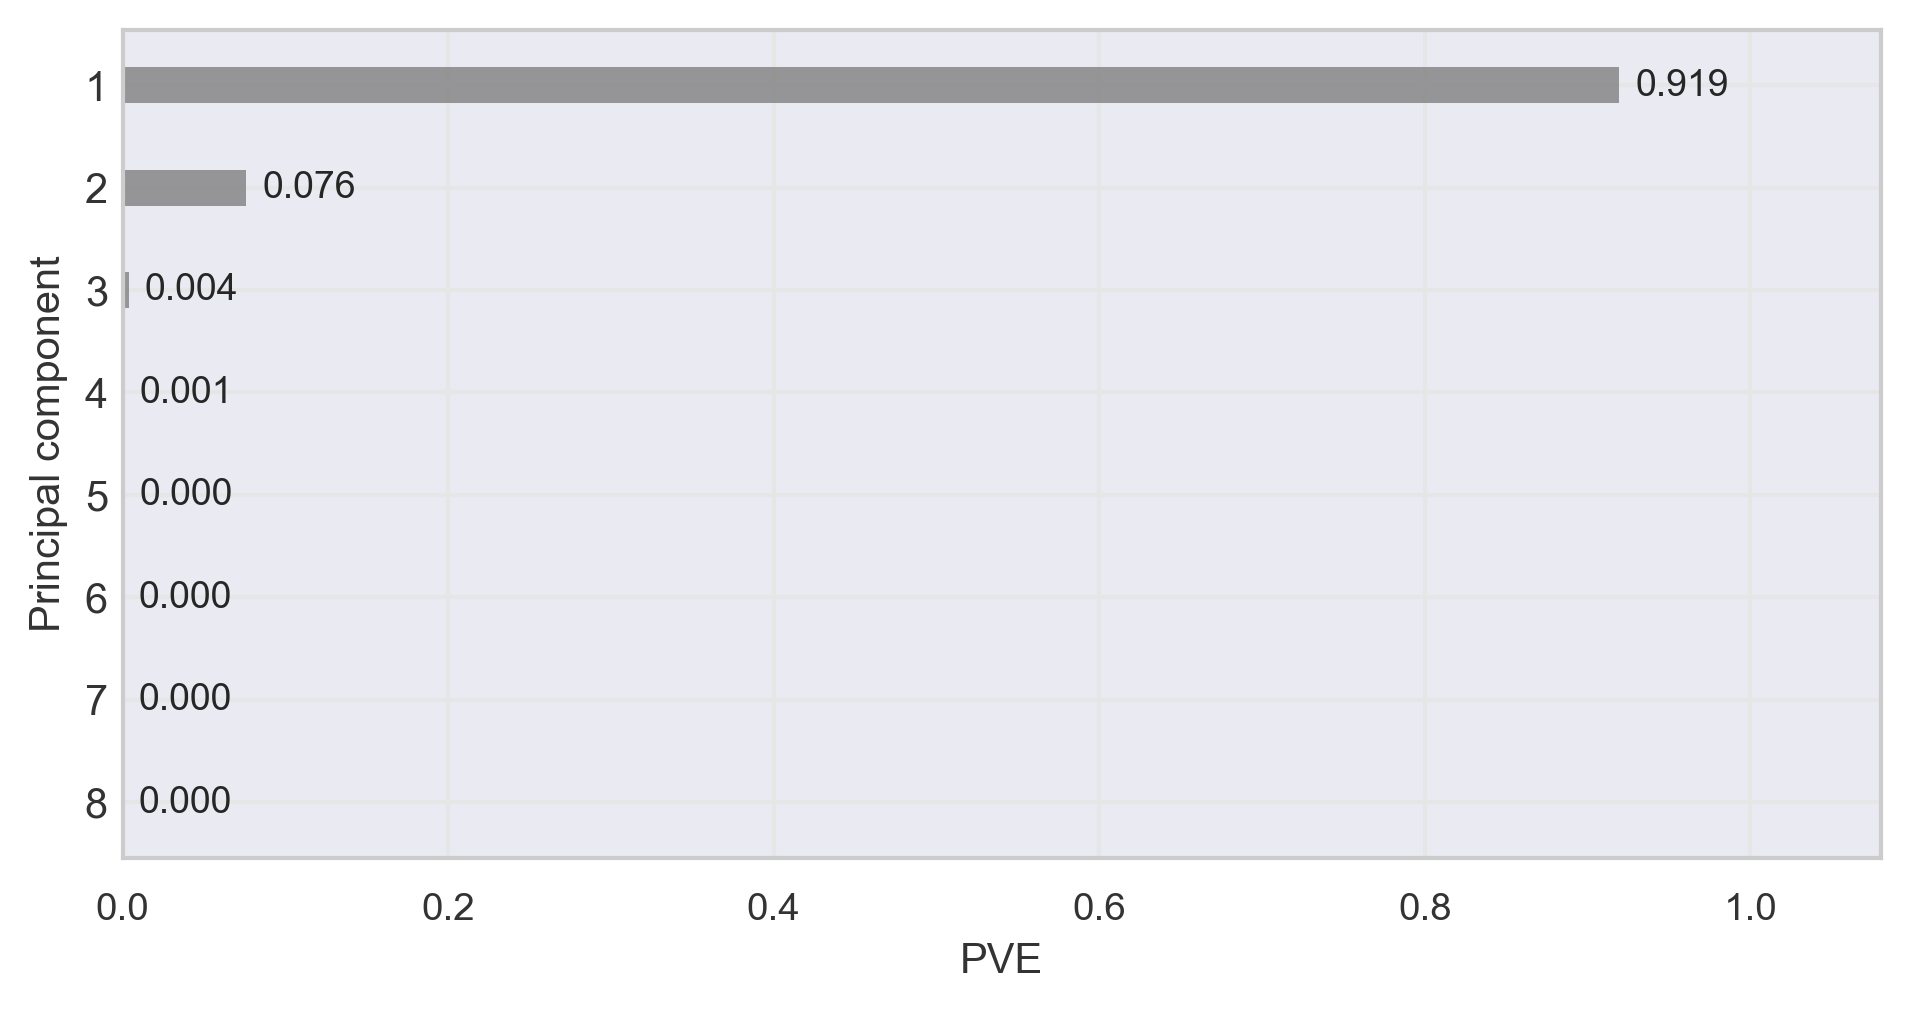
\includegraphics[width=0.55\linewidth]{Figures/thesis_results/AutoencoderPerformance/Q5b_weight_projection_barplot.png}
    \caption{Proportion of variance explained
      $\mathrm{PVE}_j = \lambda_j / \mathrm{tr}(\boldsymbol{\Sigma})$
      for each principal component, sorted in decreasing order.}
    \label{fig:pca_pve}
  \end{subfigure}

  \vspace{0.5em}

  % ── (b) Eigenvector loadings ──────────────────────────────────
  \begin{subfigure}[t]{0.48\textwidth}
    \centering
    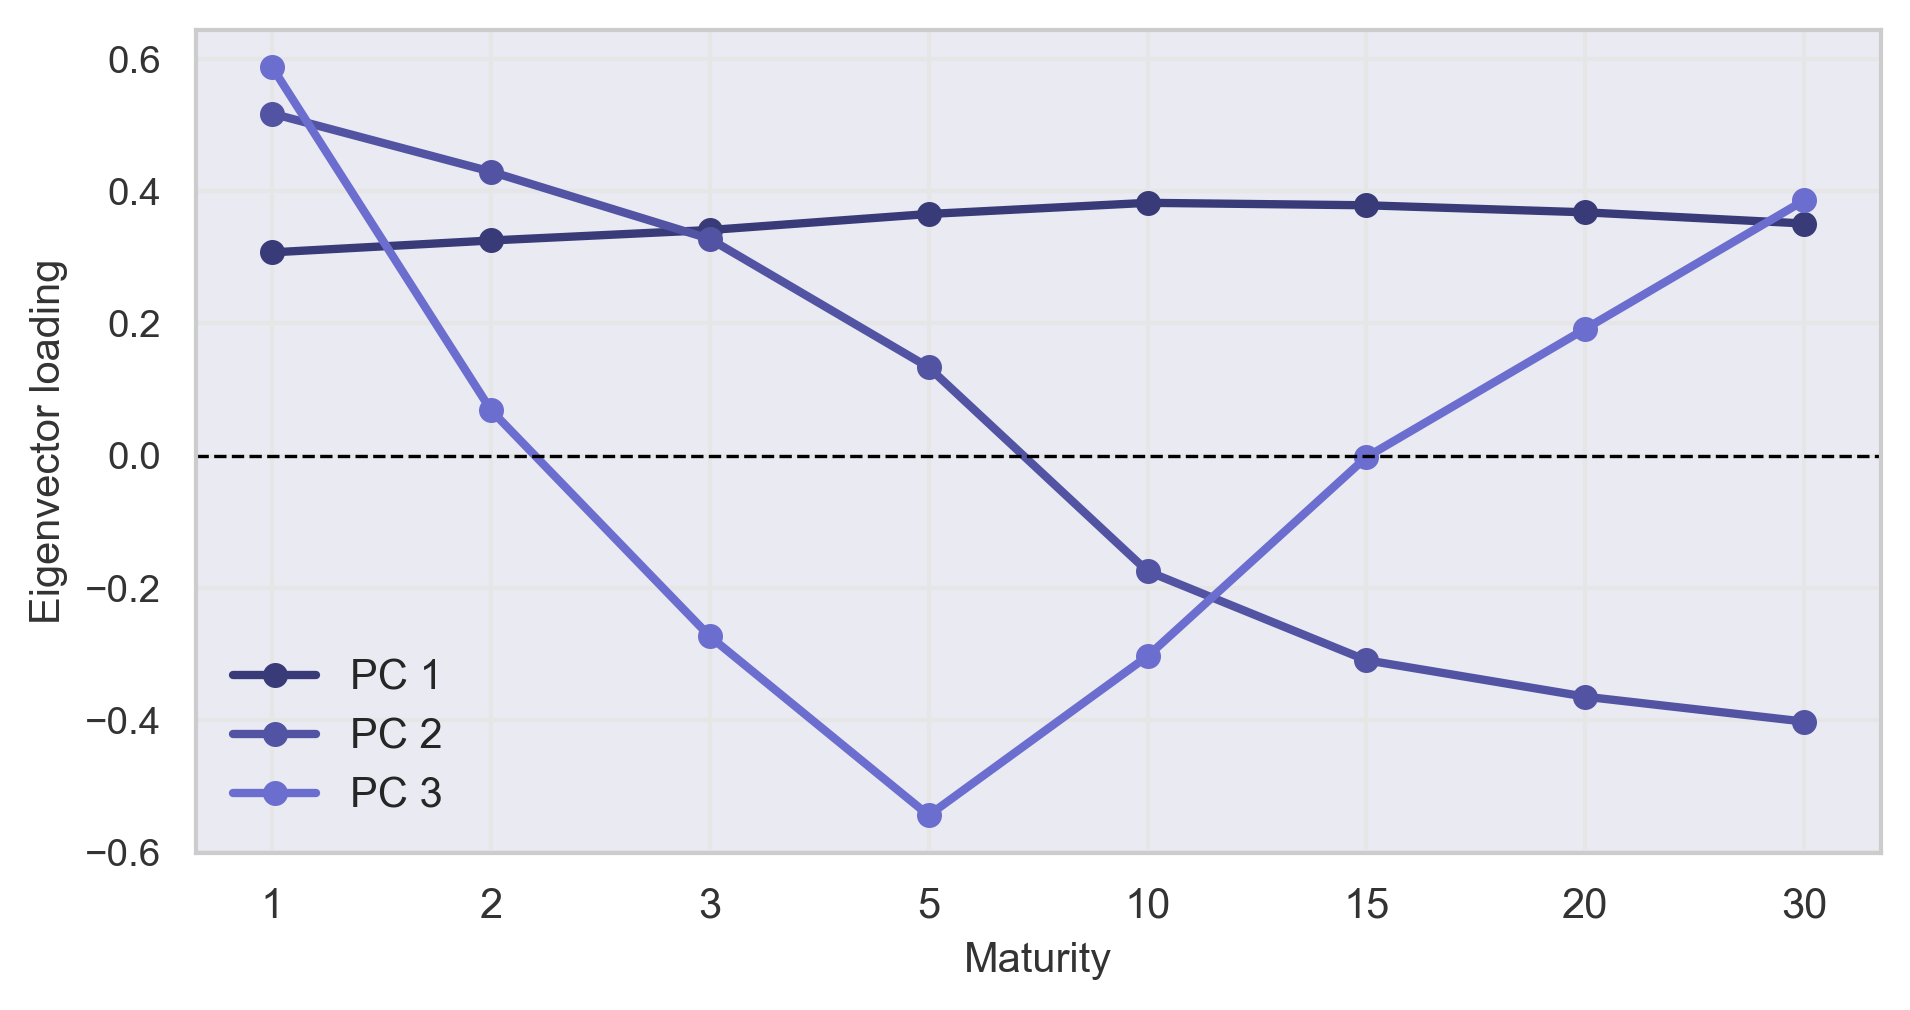
\includegraphics[width=\linewidth]{Figures/thesis_results/AutoencoderPerformance/Q5b_pca_loadings.png}
    \caption{Eigenvector loadings $\mathbf{v}_j$ across the eight
      maturities for the first three principal components.}
    \label{fig:pca_loadings}
  \end{subfigure}
  \hfill
  % ── (c) PC scores over time ───────────────────────────────────
  \begin{subfigure}[t]{0.48\textwidth}
    \centering
    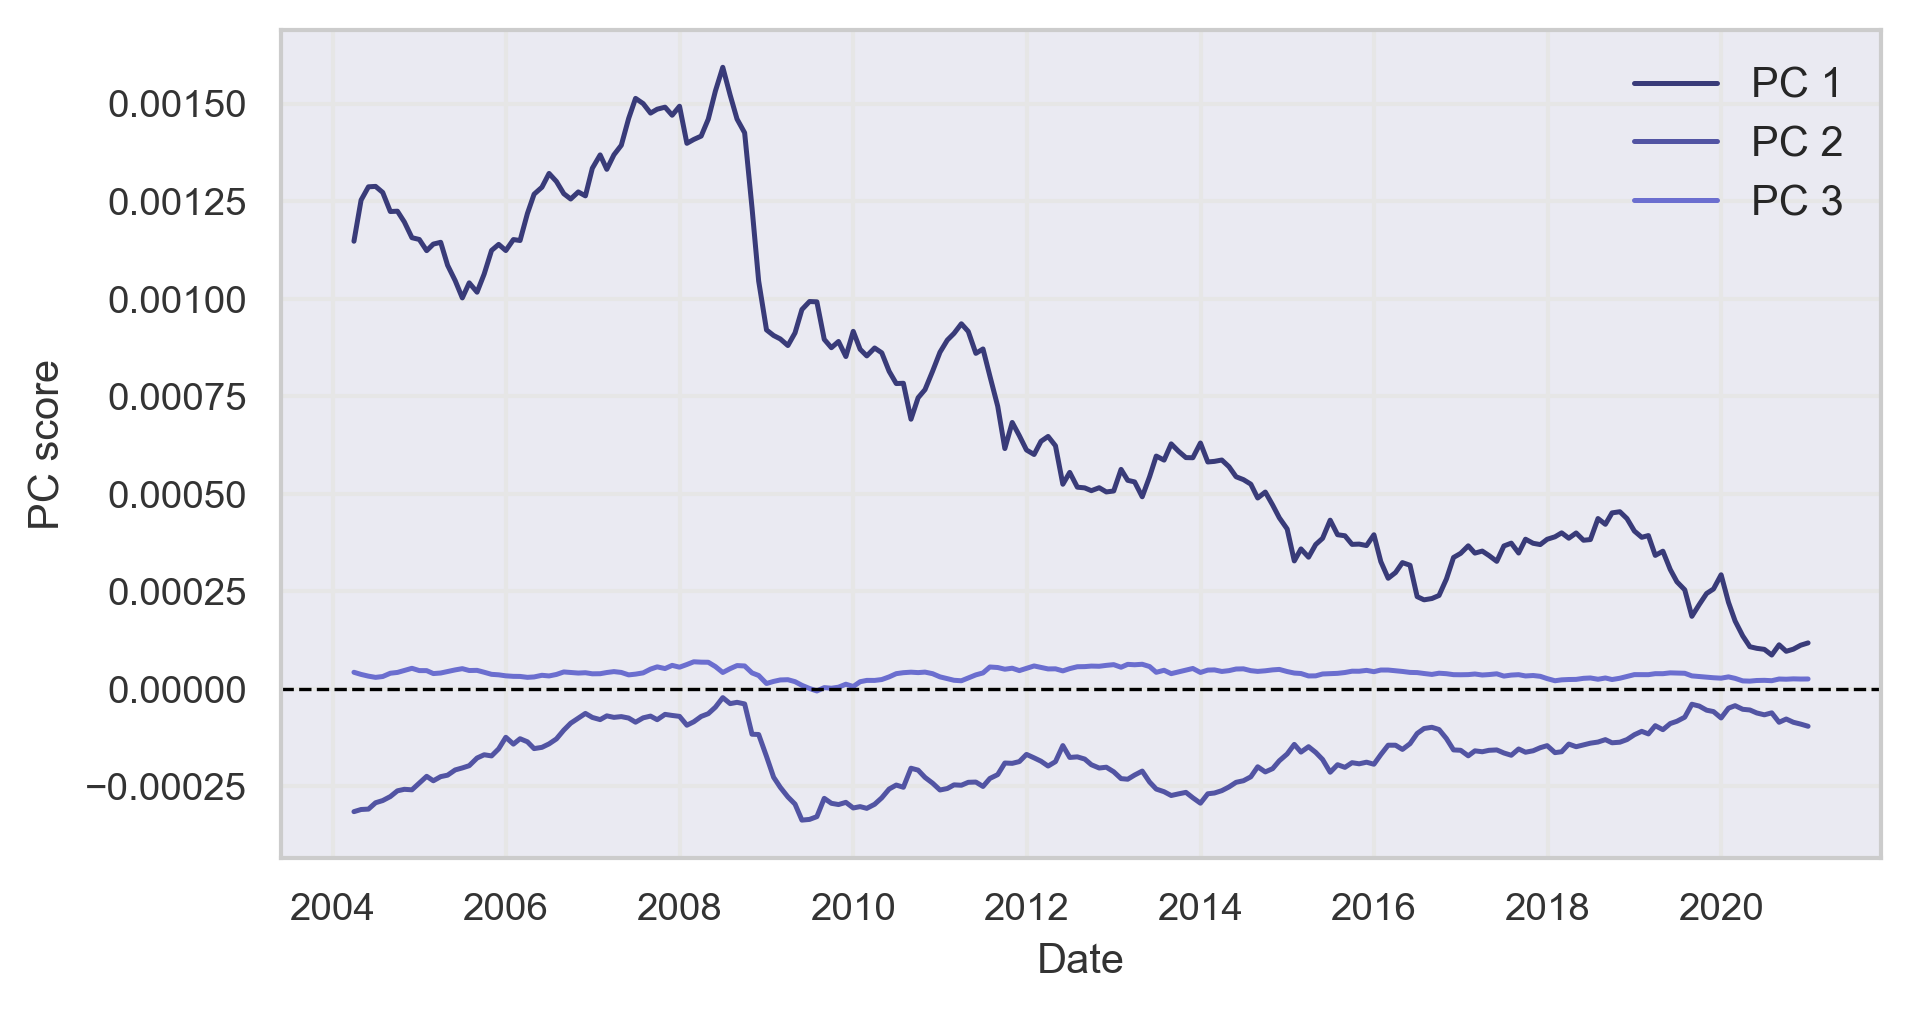
\includegraphics[width=\linewidth]{Figures/thesis_results/AutoencoderPerformance/Q5b_pca_scores.png}
    \caption{PC scores $\mathbf{v}_j^\top \mathbf{S}_t$ over time,
      averaged across currencies per date for visualisation. \textcolor{red}{Decide if its better to just visualize this for one currency instead of averaging The same with the left plot!}}
    \label{fig:pca_scores}
  \end{subfigure}

  \caption{Global PCA fitted on the pooled in-sample swap rate data
  across all nine currencies (2004--2020). PC scores in
  \subref{fig:pca_scores} are averaged across currencies per date
  for visualization.}
  \label{fig:pca_overview}
\end{figure}





Figure~\ref{fig:pca_loadings} shows the evolution of the principal
component scores over time alongside their eigenvector loadings, revealing
that the three dominant components capture the classical level, slope and
curvature structure of the swap rate curve. Having established this structure, we now ask whether the encoder has independently learned to compress the data along the same directions.




Let $\mathbf{a}_k\in\mathbb{R}^M$ denote the $k$-th row of the encoder weight matrix $A_1$, representing the direction along which factor $k$ compresses the input. Following \cite{MatinWanPoulsen2025}, we assess how much this direction aligns with each principal component $\mathbf{v}_j$ by decomposing $\textbf{a}_k$ in the PCA basis:
\begin{equation}
    w_{k,j} = \frac{(\mathbf{a}_k^\top \mathbf{v}_j)^2}{\|\mathbf{a}_k\|^2}
    \times 100, \qquad \sum_{j=1}^{M} w_{k,j} = 100.
    \label{eq:weight_proj}
\end{equation}
The projection weights for the three models across all $M=8$ principal components are presented in Table \ref{tab:weight_projection}. \textcolor{red}{Results: interpret the table here, when we have run our code}

% ── 3. Weight projection: table + bar plot + results ─────────
\pgfplotstableread[col sep=comma]{Figures/thesis_results/AutoencoderPerformance/Q5b_weight_projection_combined.csv}\wpCombined
\begin{table}[ht]
\centering
\pgfplotstabletypeset[
  col sep=comma,
  columns={model,factor,PC1,PC2,PC3,PC4,PC5,PC6,PC7,PC8},
  columns/model/.style={string type, column name={Model}},
  columns/factor/.style={string type, column name={Factor}},
  columns/PC1/.style={string type, column name={PC1}},
  columns/PC2/.style={string type, column name={PC2}},
  columns/PC3/.style={string type, column name={PC3}},
  columns/PC4/.style={string type, column name={PC4}},
  columns/PC5/.style={string type, column name={PC5}},
  columns/PC6/.style={string type, column name={PC6}},
  columns/PC7/.style={string type, column name={PC7}},
  columns/PC8/.style={string type, column name={PC8}},
  every head row/.style={before row=\toprule, after row=\midrule},
  every last row/.style={after row=\bottomrule},
  row 2/.style={before row=\midrule},
  row 5/.style={before row=\midrule},
]{\wpCombined}
\caption{Projection weights $w_{k,j}$ (in \%) of each encoder weight vector
  $\mathbf{a}_k$ onto the eight principal component directions of the
  in-sample swap rate curve, for latent dimensions $\ell \in \{2, 3, 4\}$.
  Each row sums to 100\%, following \citet{MatinWanPoulsen2025}.}
\label{tab:weight_projection}
\end{table}

The projection weights $w_{i,j}$ are purely geometric; they compare fixed directions and say nothing about whether the latent factors actually move with the PC scores through time. To assess this co-movement, we compute the Pearson correlation between factor $z_k(t)$ and the $j$-th PC score
$\mathrm{PC}_{j,t} = \mathbf{v}_j^\top \mathbf{S}_t$ over all in-sample observations:
\begin{equation}
\rho_{k,j} = \frac{\sum_{t=1}^n\bigl(z_k(t)-\bar{z}_k\bigr)
  \bigl(\mathrm{PC}_{j,t}-\overline{\mathrm{PC}}_j\bigr)}
  {\sqrt{\sum_{t=1}^n\bigl(z_k(t)-\bar{z}_k\bigr)^2
  \cdot\sum_{t=1}^n\bigl(\mathrm{PC}_{j,t}-\overline{\mathrm{PC}}_j\bigr)^2}}
\label{eq:pearson}
\end{equation}
where $\bar{z}_k$ and $\overline{\mathrm{PC}}_j$ are the respective sample
means, computed for all models $\ell \in \{2, 3, 4\}$.


Figure \ref{fig:q5b_heatmap} show the Pearson correlations $\rho_{k,j}$ for each model $\ell\in\{2,3,4\}$.\textcolor{red}{Comment} Two points of caution apply when reading the heatmap. First, the sign of each latent factor is arbitrary: any orthogonal rotation $\mathbf{R}\in O(\ell)$ applied to $z_t$ leaves the reconstruction loss unchanged, so a correlation of $-1$ is economically equivalent to $+1$. Second, a strong correlation with a PC score does not by itself confirm that the factor captures genuine market structure; it could also reflect overfitting to the training data. The out-of-sample results in Section \textcolor{red}{X} provide the complementary evidence need to distinguish between the two. \textcolor{red}{Write here a short reflection on what the correlations then represent by adding the conclusion from the OOS section.}
 
% ── 4. Correlation heatmap: AE ───────────────────────────────
\begin{figure}[ht]
  \centering
  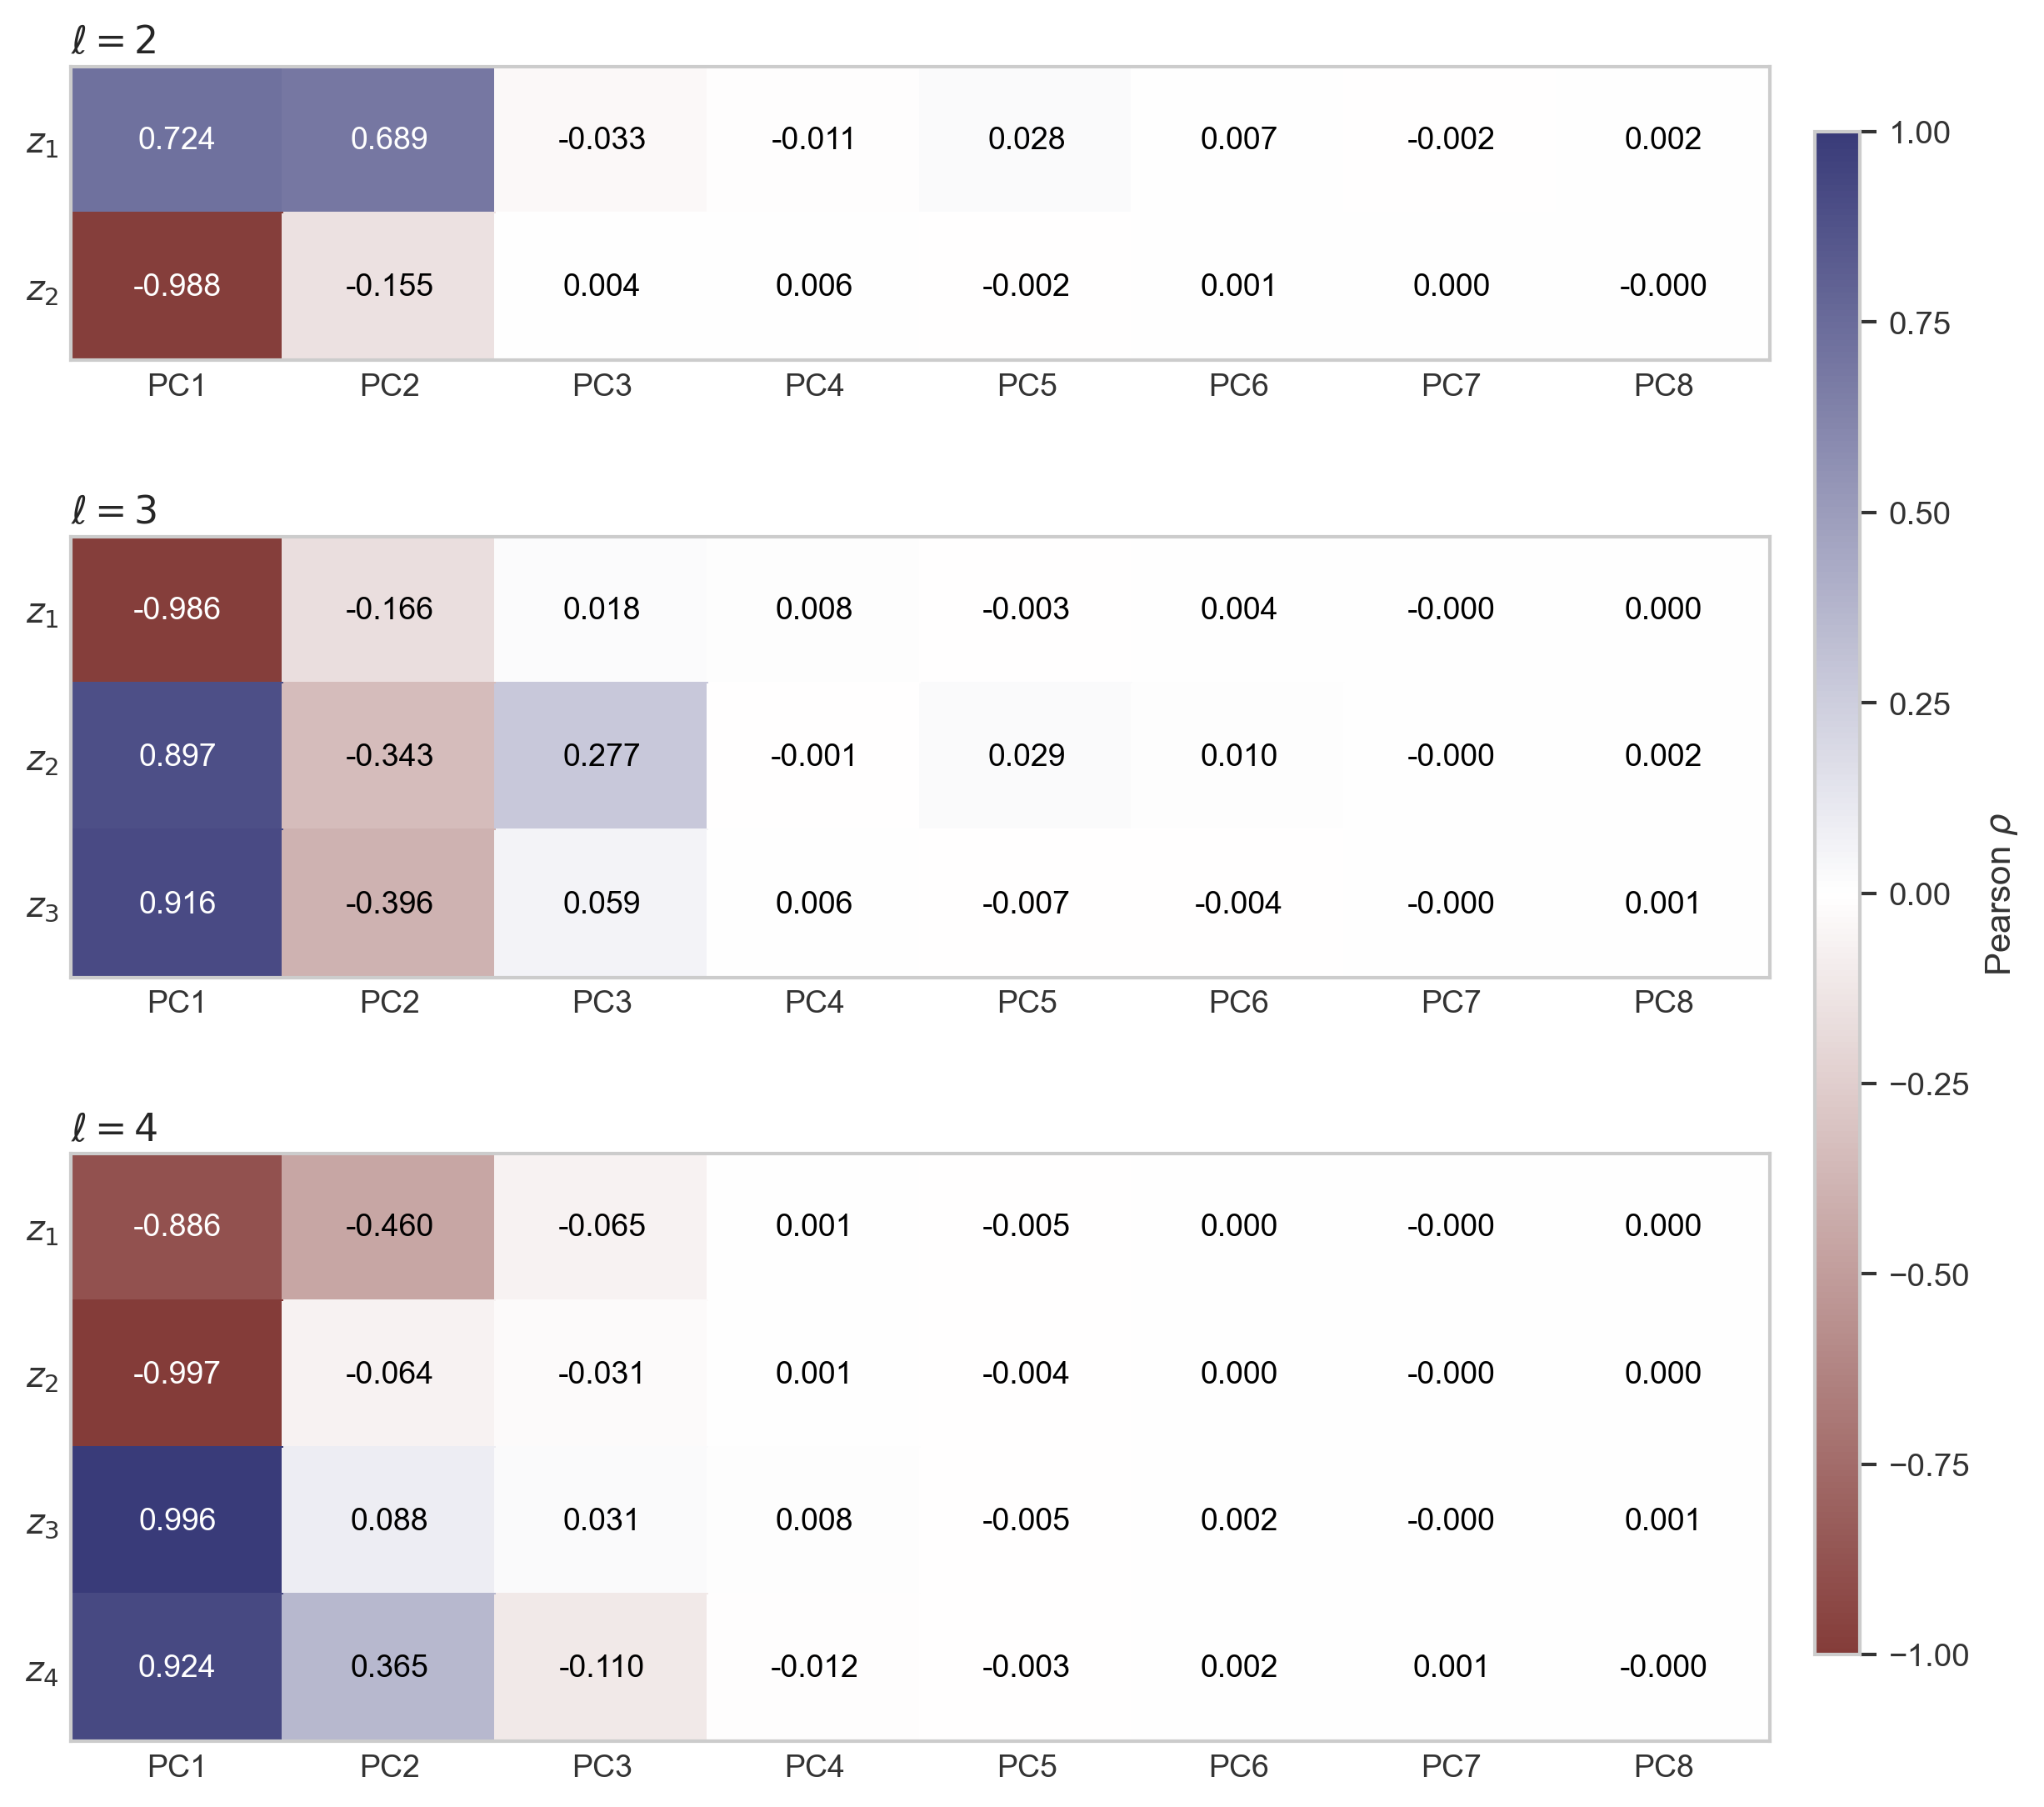
\includegraphics[width=\textwidth]{Figures/thesis_results/AutoencoderPerformance/Q5b_factor_correlation_heatmap.png}
  \caption{Pearson correlation between each autoencoder latent factor $z_k$
    and the first $\ell$ principal component scores of the in-sample swap rate
    curve, for latent dimensions $\ell \in \{2,3,4\}$.}
  \label{fig:q5b_heatmap}
\end{figure}

\textcolor{red}{Having established that the latent factors align geometrically and dynamically with the principal components}, we now examine how these factors evolve through time. Inspecting their trajectories allows us to assess whether the compressed representation captures economically meaningful variation, particularly around periods of market stress.

% ── 6. Latent factor dynamics ─────────────────────────────────
\begin{figure}[H]
    \centering
    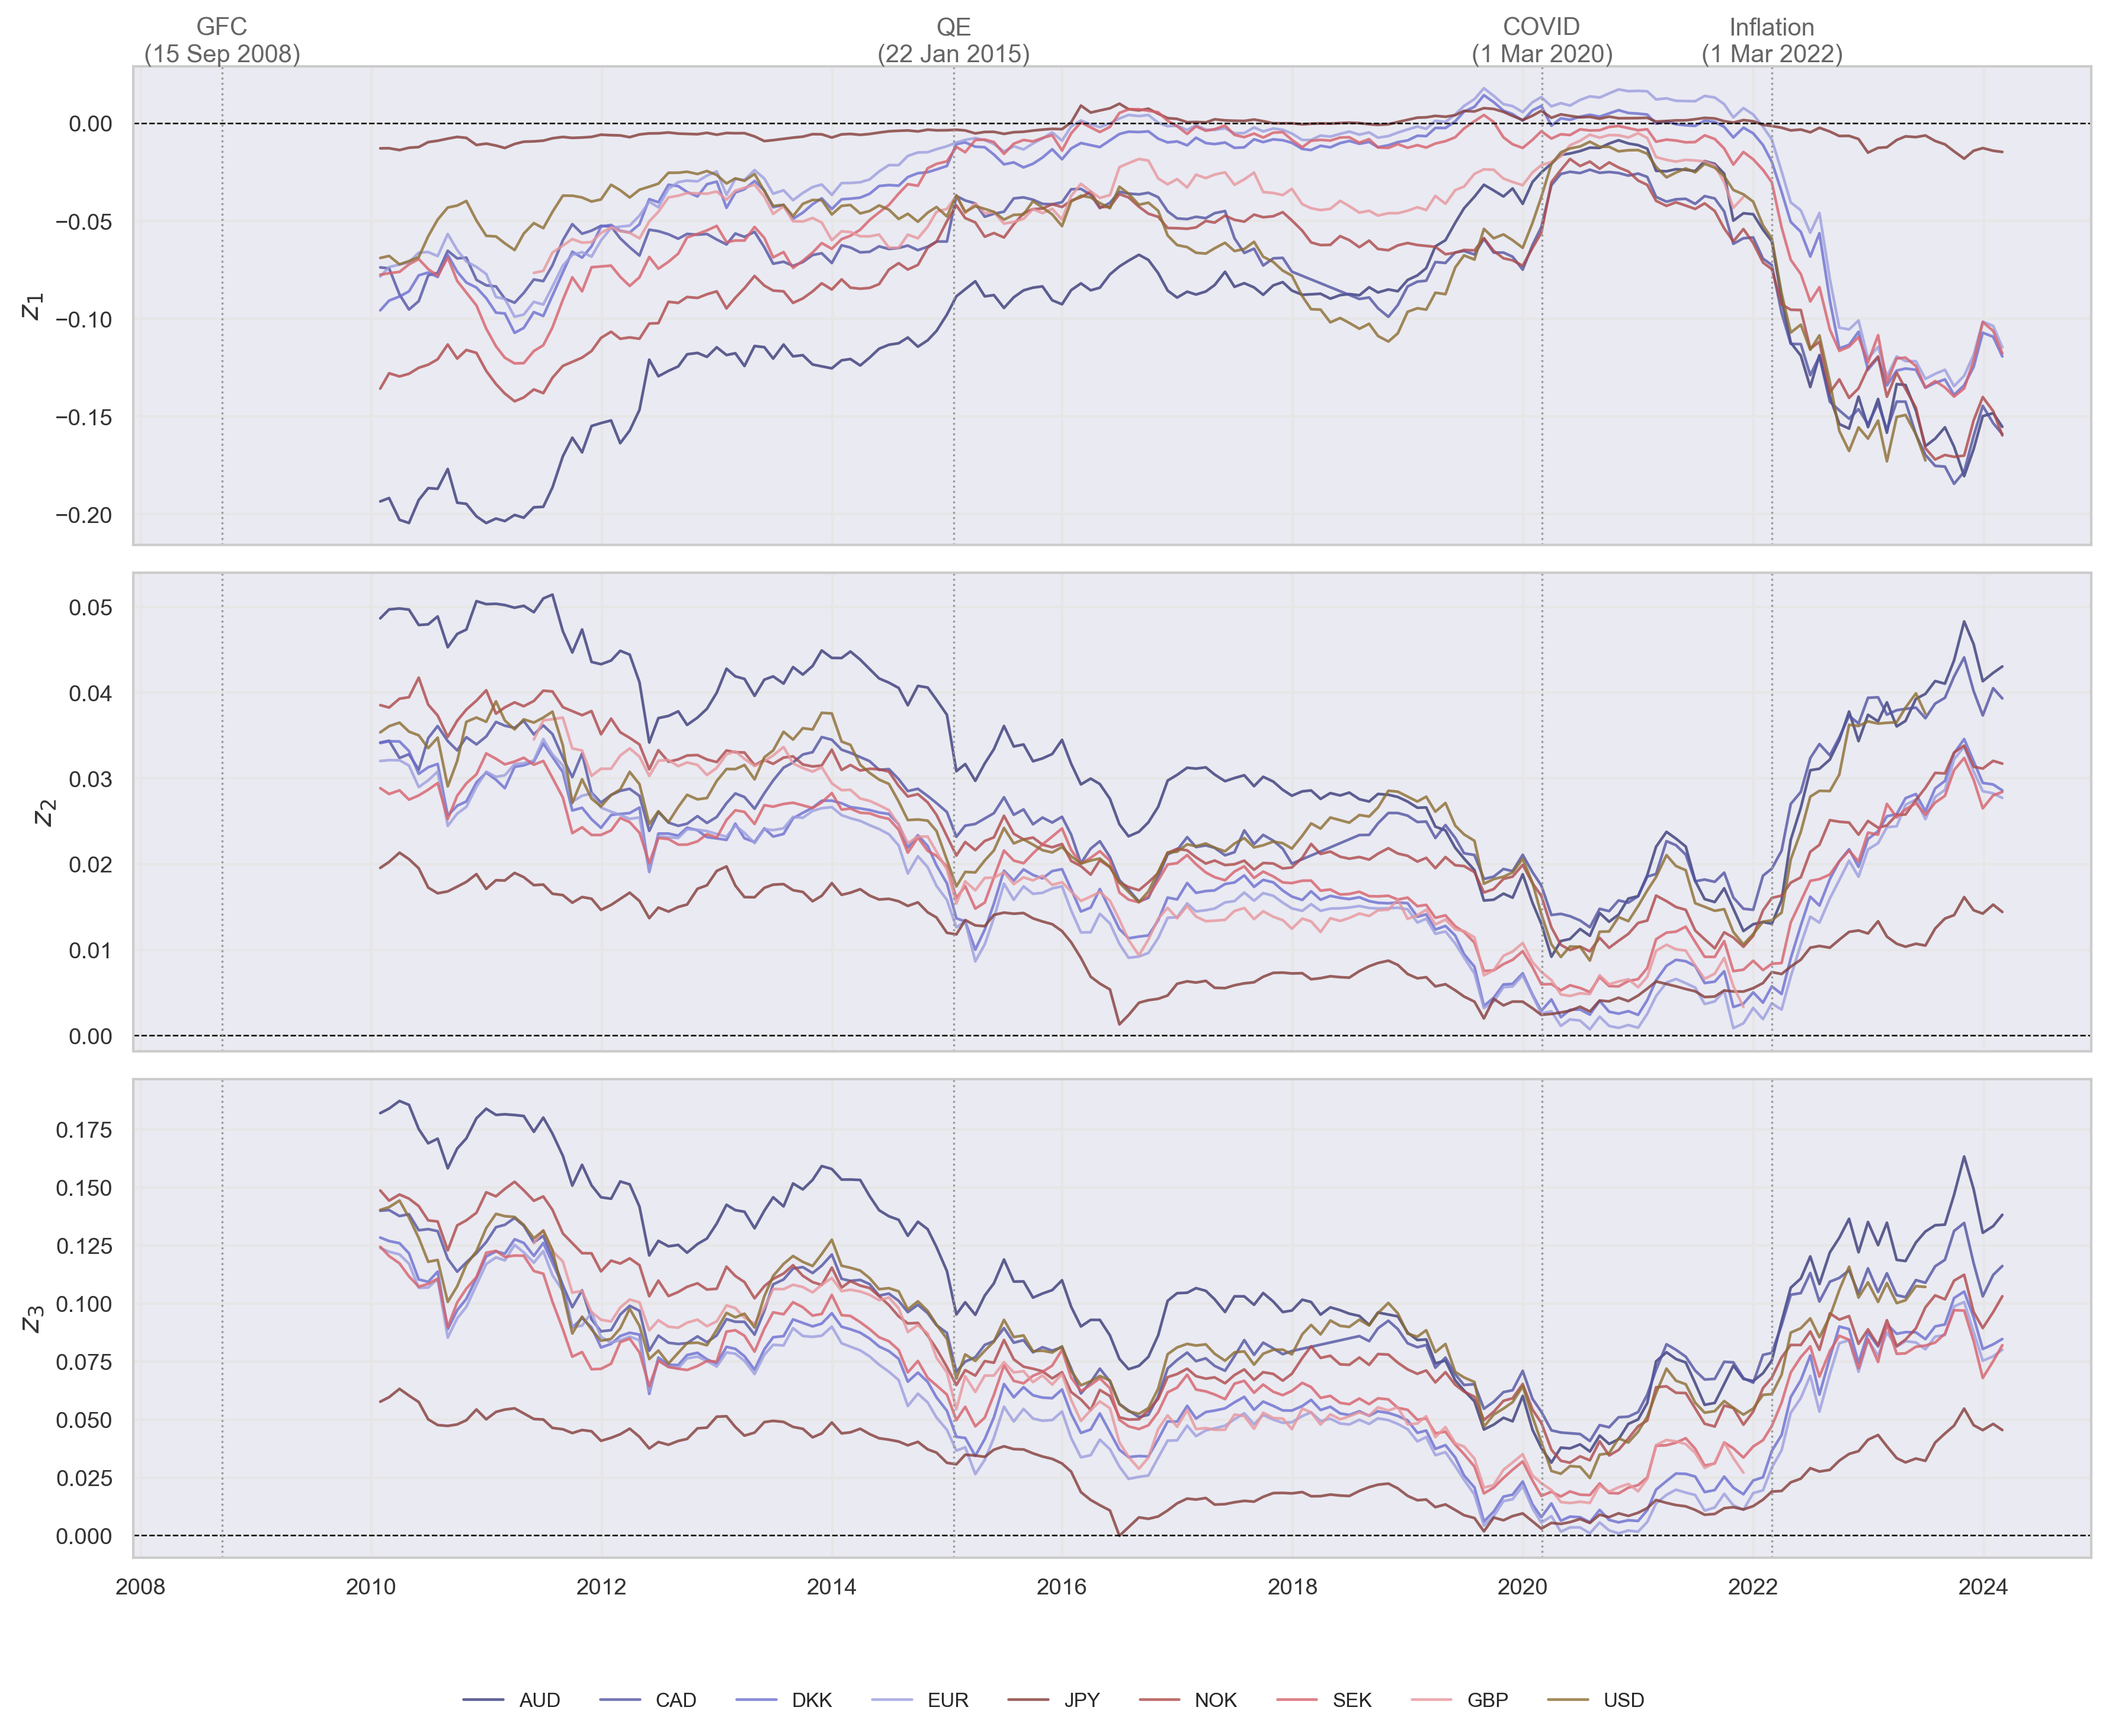
\includegraphics[width=\textwidth]{Figures/thesis_results/AutoencoderPerformance/Q5a_latent_factors_over_time.png}
    \caption{Latent factors $z_1, z_2, z_3$ over the training period
    (2004--2020) for $\ell=3$, with key market events annotated.}
    \label{fig:Q5a}
\end{figure}

The latent factor trajectories $z_1, z_2, z_3$ for the $\ell = 3$ model
over the \textcolor{red}{full in-sample period 2004--2020} are shown in
Figure~\ref{fig:Q5a}. The factors exhibit distinct low-frequency trends
punctuated by sharp transitions around the major market dislocations:
the Global Financial Crisis (2008--2009), the ECB quantitative easing
programme (2015--2018), and the COVID-19 shock (2020).
\textcolor{red}{Comment}


\textcolor{red}{Sum up here when results are updated.}







\section{Implied Yield curve}

We now want to assess how it visually reconstructs, and if it replicates the shape well, something that A metrics such as RMSE does not reveal.


\begin{figure}[H]
    \centering
    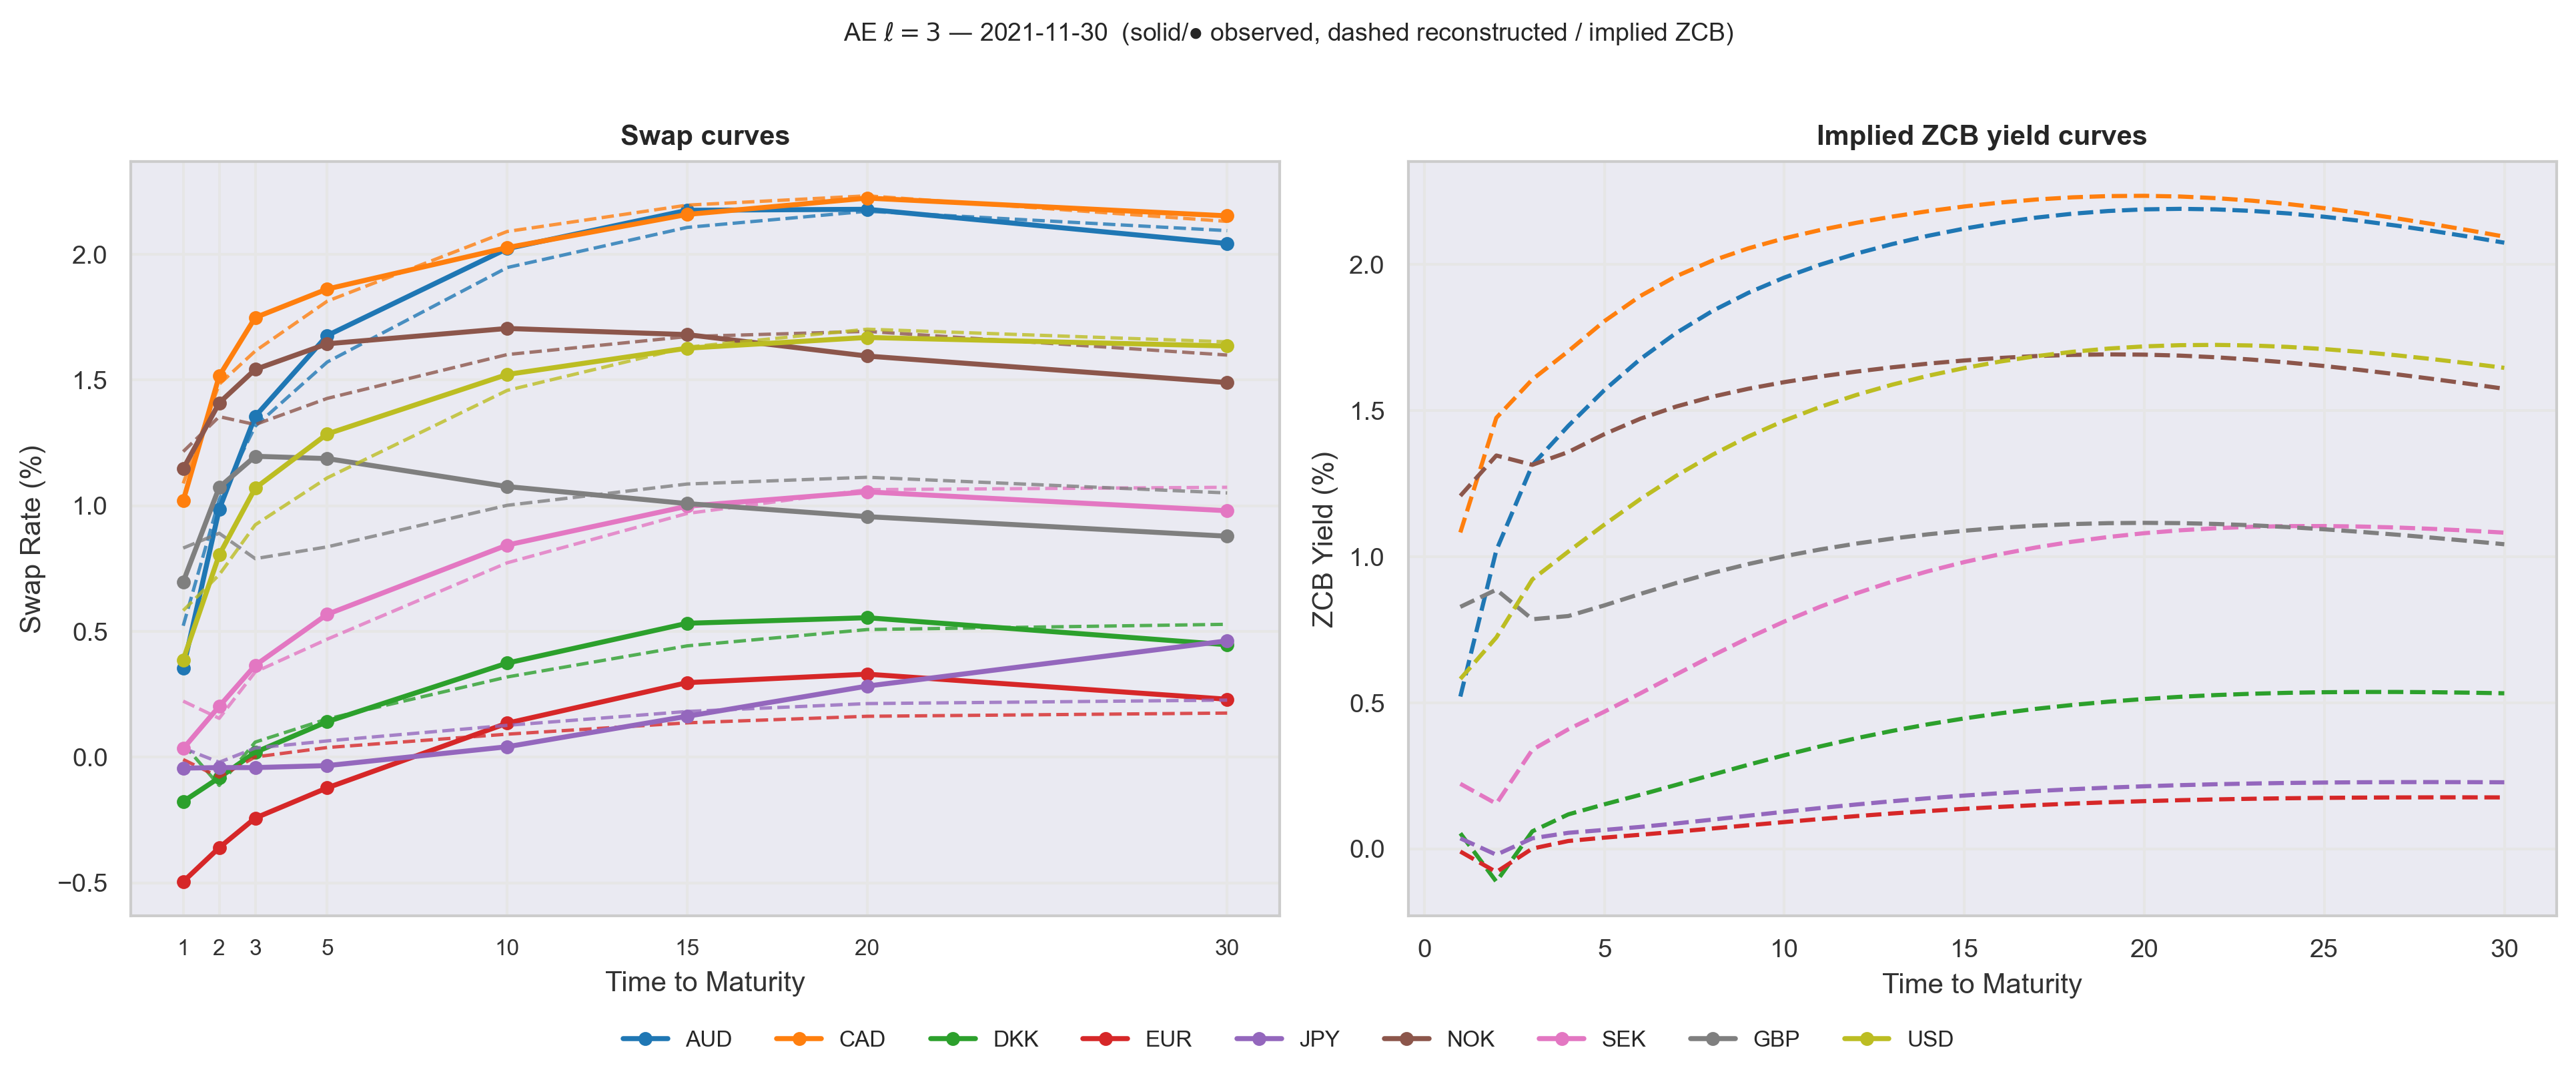
\includegraphics[width=1.0\textwidth]{Figures/thesis_results/AutoencoderPerformance/Q1e_zcb_swap_dim3.png}
    \caption{Swap curves and implied zero-coupon bond (ZCB) yields for the
    autoencoder ($\ell=3$) on 30 November 2021.
    Left panel: observed swap rates (solid with circles) and reconstructed
    swap rates (dashed). Right panel: ZCB yields implied by the model,
    computed as $y(\tau) = -\log P(0,\tau)/\tau$.
    Currencies:
    AUD ({\color[HTML]{393B79}\rule[0.5ex]{1em}{1.5pt}}),
    CAD ({\color[HTML]{5254A3}\rule[0.5ex]{1em}{1.5pt}}),
    DKK ({\color[HTML]{6B6ECF}\rule[0.5ex]{1em}{1.5pt}}),
    EUR ({\color[HTML]{9C9EDE}\rule[0.5ex]{1em}{1.5pt}}),
    JPY ({\color[HTML]{843C39}\rule[0.5ex]{1em}{1.5pt}}),
    NOK ({\color[HTML]{AD494A}\rule[0.5ex]{1em}{1.5pt}}),
    SEK ({\color[HTML]{D6616B}\rule[0.5ex]{1em}{1.5pt}}),
    GBP ({\color[HTML]{E7969C}\rule[0.5ex]{1em}{1.5pt}}),
    USD ({\color[HTML]{8C6D31}\rule[0.5ex]{1em}{1.5pt}}).}
    \label{fig:Q1e_zcb}
\end{figure}




